\section{Introduction}

In Bitcoin~\cite{bitcoin}, a population of \emph{miners}
attempt to find \emph{blocks} in the form $B = h \concat x \concat ctr$,
where $h$ is a pointer to the previous block, $x$ contains a sequence of
\emph{transactions}, and $ctr$ is a \emph{nonce}. The nonce is brute forced
by the miner to satisfy the \emph{proof-of-work} inequality $H(B) < T$, where
$H$ is a hash function with output in the interval\footnote{The deployed hash function of, e.g., Bitcoin,
is SHA-256, which outputs a $256$-bit string. The value can be scaled to the interval $(0, 1)$ by
dividing by $2^{256}$.}
$(0, 1)$
and $T$ is a small \emph{target} in the interval $(0, 1)$. Any $B$ that satisfies this
inequality is considered a \emph{valid block}, whereas candidates that do not satisfy
the inequality are invalid. Simply put, valid blocks must have
hashes that begin with a desired number of $0$s.
These blocks form linked lists known as \emph{chains}.
Among such chains, the \emph{heaviest} chain is chosen as the canonical one.

Some blocks $B$ satisfy the proof-of-work inequality better than others.
Namely, they satisfy not only $H(B) < T$, but also $H(B) < \frac{T}{2^w}$
for some $w \in \mathbb{R}^+$. Nevertheless, these heavier blocks are counted all the same when choosing
which chain to pick.
We posit that the weight of a block is information
that can be useful to improve the protocol.
In this paper, we introduce \emph{\poem}.
We modify the fork choice rule of Bitcoin to take this information into account.
We build a protocol which retains the same level of security as Bitcoin, while achieving
better confirmation latency or transaction throughput, because the number of confirmations
can be safely reduced, or the block production rate can be safely increased respectively.

We report on our production implementation of a real-world system
in which we employ this new rule, and show that it achieves a $28.5\%$
improvement in confirmation latency
or a $16.3\%$ improvement in throughput as compared to Bitcoin.
We also theoretically prove our new protocol is secure
using the Bitcoin Backbone model. Our theoretical analysis introduces
a new technique, the \emph{real-valued random oracle}, which we prove behaves
similarly to the usual random oracle. This variant of the
random oracle allows for the use of an arsenal of theoretical tools from the
continuous domain (such as continuous distributions), easing the theoretical
exposition, and may be of independent interest.

\noindent
\myparagraph[Construction overview]
The classical Bitcoin protocol uses the heaviest chain fork choice. Among two different
chains, the one with the \emph{most work} is chosen as the canonical one, where the work (or difficulty) of a block
is defined as $\frac{1}{T}$, with $T$ being the mining target. We modify this
rule as follows: Each block counts for its \emph{intrinsic} work $-\lg \frac{H(B)}{T}$,
where $H(B)$ denotes the hash of the block. Intuitively, this corresponds to counting the
``number of extra zeroes'' at the front of the actually achieved hash of each block, not just accounting
for its nominal target. The zeroes at the front of the hash are already guaranteed
to be at least $-\lg T$, but can be more. The score of each block is \emph{how many extra zeroes}
it has. The chain with the most total intrinsic work is chosen as the canonical chain.

\iftwocolumn
\begin{figure*}
  \centering
  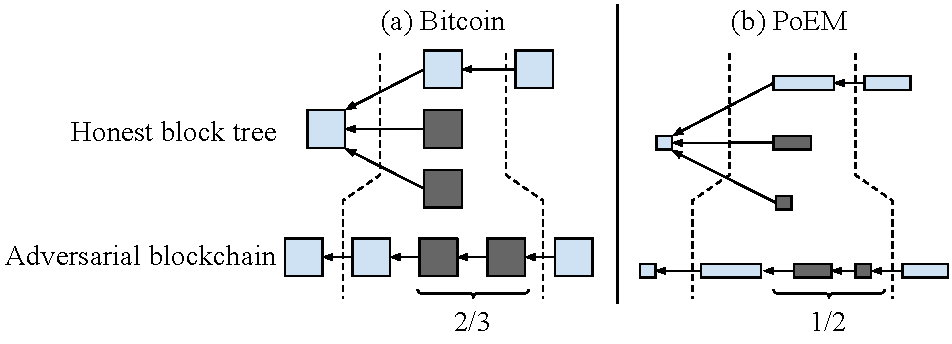
\includegraphics[width=0.6\textwidth,keepaspectratio]{figures/poem_work_wasted.pdf}
  \caption{The same block mining successes awarded to the honest parties (top) or the adversary (bottom)
           with equal mining power on Bitcoin (left) or PoEM (right) respectively. The adversary can place
           all blocks in one sequence because she does not incur any network delay. The honest parties,
           due to the delay, may place blocks at the same height (dashed section of duration $\Delta$).
           In this example, when $3$ honest blocks were found almost simultaneously, $2$ out of
           them were abandoned in Bitcoin and did not make it to the canonical longest chain
           (top-most chain).
           In the PoEM example, $2$ out of $3$ of the honest blocks were abandoned, but the cumulative intrinsic
           work wasted only happened to be $1/2$ of the intrinsic work produced during this interval.
           We illustrate the intrinsic work of a block by its size.}
  \label{fig:poem-wasted-work}
\end{figure*}
\else
\begin{figure*}
  \centering
  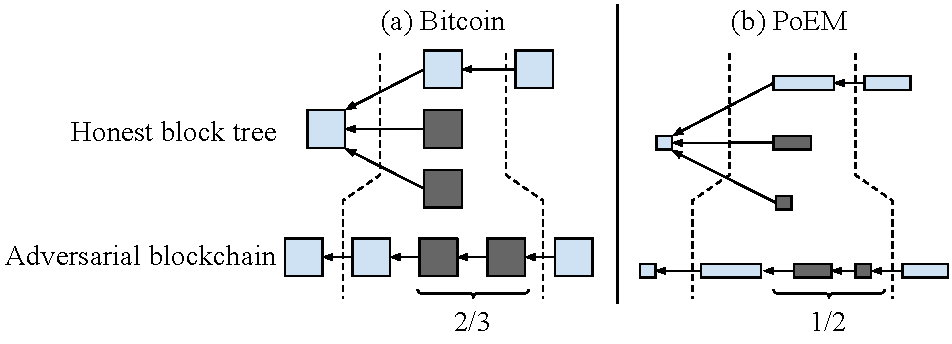
\includegraphics[width=0.8\textwidth,keepaspectratio]{figures/poem_work_wasted.pdf}
  \caption{The same block mining successes awarded to the honest parties (top) or the adversary (bottom)
           with equal mining power on Bitcoin (left) or PoEM (right) respectively. The adversary can place
           all blocks in one sequence because she does not incur any network delay. The honest parties,
           due to the delay, may place blocks at the same height (dashed section of duration $\Delta$).
           In this example, when $3$ honest blocks were found almost simultaneously, $2$ out of
           them (shaded) were abandoned in Bitcoin and did not make it to the canonical longest chain
           (top-most chain).
           In the PoEM example, $2$ out of $3$ of the honest blocks were abandoned, but the cumulative intrinsic
           work wasted only happened to be $1/2$ of the intrinsic work produced during this interval.
           In PoEM (right), we illustrate the intrinsic work of a block by its size.}
  \label{fig:poem-wasted-work}
\end{figure*}
\fi

To see the benefits of this rule, first observe that it provides a natural tie-breaking rule:
If two honest parties observe the same block tree, they will agree on
the canonical chain, regardless of the order of network message arrival. The \poem protocol
outperforms Bitcoin when the block production rate is increased. It is generally desirable
to increase the block production rate, because it corresponds to an increase in the chain growth
rate, which, in turn, increases the transaction throughput.
However, when the expected block interarrival time approaches the network delay, multiple honest blocks
can be produced in short succession without allowing for honest nodes to synchronize their views.
As a result, multiple honest nodes may produce blocks at the same height, and only one of these will
eventually make it to the canonical chain, while the others will be discarded. These discarded blocks
do not contribute to the growth of the length of the honest chain. Our protocol is similar to Bitcoin in that,
whenever multiple honest blocks are found simultaneously, only one of them survives in the canonical chain,
and the rest are discarded. However, the surviving block is the \emph{heaviest} block among them, in terms of intrinsic
work, as illustrated in Figure~\ref{fig:poem-wasted-work}. Hence, the discarded
work is less. This gives an advantage to the honest
parties when they are racing against a private mining attacker, since they can produce chains that grow
at a faster rate. This intuition generalizes to arbitrary adversaries.
The small change we introduce in the fork choice rule allows us to safely increase the block production
rate, as compared to Bitcoin, without sacrificing adversarial resilience. The resulting protocol
allows for faster transaction confirmation, or better throughput, while retaining the same level of security.

\noindent
\myparagraph[Related work]
Bitcoin was first proven secure in the static population setting~\cite{backbone},
and later also studied in the variable population setting~\cite{varbackbone}.
The idea of using a more nuanced proof-of-work inequality in which some blocks
are considered heavier than others was first put forth by Andrew Miller~\cite{highway},
with the first complete protocol to utilize it being
Proofs of Proof-of-Work~\cite{popow}. These were later refined multiple times
to account for non\-/interactivity~\cite{nipopows}, backwards compatibility~\cite{velvet-nipopows},
onlineness~\cite{logspace}, on-chain data efficiency~\cite{compact-superblocks},
gas consumption~\cite{gasefficient-nipopows},
bribing resilience~\cite{soft-power},
and variable populations~\cite{dionyziz}.
We are the first to modify the fork choice rule to take these refinements into
account, following \ifanonymous
the
\else
our
\fi
previous short paper ``POEM: Proof of Entropy Minima''~\cite{poem-short},
where the entropic fork choice rule was defined but not analyzed.
Our work only changes the PoW inequality.
Other mechanisms refining the fork choice rule
are orthogonal and can be combined with our approach, yielding even
further performance gains.
Such examples include
PHANTOM~\cite{phantom}, SPECTRE~\cite{spectre}, GhostDAG~\cite{ghostdag}, and
GHOST~\cite{ghost}.
Additional mechanisms towards improving the latency and throughput
of proof-of-work blockchains at the consensus
layer, also composable with ours, include parallel chains~\cite{parallel-chains},
separation of transaction/consensus blocks~\cite{prism},
hybrid approaches between proof-of-work and proof-of-stake~\cite{byzcoin},
and the use of microblocks~\cite{bitcoin-ng}.